\vfill\null

\section{STEREOFONIA}

Prima di arrivare al concetto elettroacustico ed alle tecniche legate alla
\emph{Stereofonia} è necessario stabilire, attraverso l'etimologia del termine,
e dei termini ad esso collegati, una base concettuale solida. \emph{Stereo},
dal greco \emph{Stereos}, significa \emph{solido}. Non un numero, non una
configurazione ma un aggettivo qualitativo. Solido, nel dizionario inglese
\emph{Solid, firm and stable in shape. Having Three dimension.} Solido,
\emph{solid}, dalla radice latina di \emph{Solidus, Sollus}, intero.

Con la parola \emph{Stereofonia} dovremmo quindi descrivere una condizione
nella quale \emph{phon\={e}}, sempre dal greco, \emph{suono}, la \emph{voce},
arrivi all'ascoltatore solida, integra, ferma e stabile nella sua forma (sonora)
multi dimensionale, intera.

Indispensabile alla comprensione del mondo sonoro elettracustico, nelle sue
radici, è anche la descrizione di \emph{mono}, nomignolo di \emph{monofonico},
espresso nel legame tra \emph{monos} e \emph{phon\={e}}: una voce,
\emph{one voice}, \emph{alone}. La stessa parola usata nella descrizione del
canto gregoriano, successivamente evolutasi in \emph{polifonia} (dal greco
\emph{poluph\={o}nia}, da \emph{polu}, molte, \emph{many} e \emph{phon\={e}},
voci). Quindi la dicotomia, se proprio deve essercene una, tra monofonia e
stereofonia semplicemente non esiste. L'estensione del concetto di monofonia è
la polifonia. La stereofonia è semplicemente un concetto altro.

Con la parola stereofonia dovremmo descrivere anche la condizione in base alla
quale il suono arrivi \emph{solido} all'ascoltatore, \emph{whole}, \emph{fermo e
stabile} nella loro sua forma sonora multidimensionale originaria, anche nella
sua riproduzione elettroacustica, con un numero qualsiasi necessario di canali.

\clearpage

%%%%%%%%%%%%%%%%%%%%%%%%%%%%%%%%%%%%%%%%%%%%%%%%%%%%%%%%%%%%%%%%%% SECTION THREE
%%%%%%%%%%%%%%%%%%%%%%%%%%%%%%%%%%%%%%%%%%%%%%%%%%%%%%%%%%%%%%%%%%%%%%%%%%%%%%%%
\section{LE RADICI}

Il sano atteggiamento mentale nei confronti della condivisione della conoscenza
prevede le radici della conoscenza e della condivisione, anche senza
interpretazioni, che potrebbero essere fornite in seguito.

\begin{quotation}
An observer in the room is listening with two ears, so that echoes reach him
with the directional significance which he associates with the music performed
in such room. He therefore discount these echoes and psychologically focuses
his attention on the source of the sound. When the music is reproduced through
a single channel the echoes arrive from the same direction as the direct sound
so that confusion results. [\ldots] Human ability to determine the direction
from which sound arrives is due to binaural hearing, the brain being able to
detect differences between sound received by the two ears from the same source
and thus to determine angular directions from which various sounds arrive.
\cite{ab58}
\end{quotation}

Con queste parole, Blumlein ha descritto i fondamenti di almeno due grandi argomenti: come percepiamo i suoni acustici e come abbiamo riprodotto i suoni fino a quel momento per essere ascoltati e percepiti.

L'ascolto binaurale umano è la prima affermazione del concetto di Blumlein: “\emph{un osservatore nella stanza sta ascoltando con due orecchie}”. Come questa condizione di ascolto si evolva nel tempo è la peculiarità della stereofonia. Non è correlato al numero di fonti, nemmeno al numero di microfoni e altoparlanti necessari per riprodurre tale condizione. La tecnica e lo scopo della tecnica prescelta si concentreranno per risolvere più argomenti possibili per soddisfare tale condizione.

Una singola voce umana sta parlando, una voce monofonica all'interno di una piccola stanza, una condizione stereofonica accettabile? In accordo con Blumlein, Sì! Questo è il primo punto fermo.

Michael Gerzon, dagli anni settanta agli anni novanta, dalle radici dell'era di Blumlein ha saltato la linea con una dozzina di descrizioni chiare sulla percezione e tentativi di progettare tecnologie di riproduzione per colmare il divario rispetto al regno acustico.

\begin{quotation}
The ears and brain localize sounds according to many different mechanism. Among the most important cues used are low frequency interaural phase (applicable up to around 2\emph{KHz}, but dominant below 700\emph{Hz}) and localization by amplitude differences between the two ears, predominantly above about 1\emph{KHz}. While other cues are also important, we have found that satisfying both these cues, and making them mutually consistent for central listener facing in any direction, leads to particularly robust and reliable localization quality.\cite{mg92pdmsss}
\end{quotation}
%
% \vfill\null
%
% \newpage
%
% %%%%%%%%%%%%%%%%%%%%%%%%%%%%%%%%%%%%%%%%%%%%%%%%%%%%%%%%%%%%%%%%%%% SECTION FOUR
% %%%%%%%%%%%%%%%%%%%%%%%%%%%%%%%%%%%%%%%%%%%%%%%%%%%%%%%%%%%%%%%%%%%%%%%%%%%%%%%%
% \section{Branches}
% \label{sec:branches}
%
% With the deep knowledge of time meaning between us and Blumlein, we can expose loudspeaker significance better than him. For the Blumlein era, the loudspeaker was the future instrument for a better present time. The reproduced sound, at its young age, was pure magic. Today we know well how unsatisfied we are of loudspeaker reproduction. When the first iPhone was the only one smart-thing on the planet, it was awesome, an awesome object of crafting. Today with the same object we would not take even a picture. Listening to a violin solo reproduced by the best loudspeaker on the market is not the same experience of the real performance. It is not related to stereophony and technique ability, it is integral to the reproduction limit of the technology we are able to craft.
%
% Replacing the human voice speaking of the example before, with a single loudspeaker speaking the recordings of that human voice we lose, as Blumlein described, the capacity of ears-brain deciphers the sound-environment relationship. It is not more the same stereophonic listening. The numbers of sources are the same. Both of them in their monophonic speaking produce a different listening condition.
%
% In 1992 Michael Gerzon \cite{mg92pdmsss} draws a schematic representation of different loudspeakers positions for multispeaker stereo, from one to five:
%
% \begin{quotation}
% \ldots we show the loudspeaker layouts considered for frontal stage stereo using from one (regarding mono as the trivial case of “one-loudspeaker stereo”!) to five loudspeakers…
% \end{quotation}
%
% Is there a one-loudspeaker stereo condition? Truly yes.
%
% A loudspeaker in condition to play itself, not reproducing something of acoustic real but \emph{producing} a sound that not could live without a loudspeaker, represents a stereo condition with general characteristics similar to the speaking voice. A Butterworth filtered pink noise monophonically singing in a room is a condition of stereophony.
%
% For an electroacoustic musician, the loudspeakers are instruments. Choosing loudspeakers, knowing their character and their characteristics is a necessary moment for that musician. Knowing their character requires time. Manually changing the frequency of a sinusoidal sound reproduced by a three-way loudspeaker, at one meter of distance, with the ears at the same high of the loudspeaker center, is a good way to say Hello! at the loudspeaker. The musician will discover in this way that the sounds produced by the loudspeaker will change their shape during the sweeping. Near the crossing point of the crossover maybe He will find some peculiarities, some other strange phase decorrelations at very high frequency. The loudspeakers are instruments. Two loudspeakers could be the minimum set for the stereophonic condition of listening. They could be polyphonic electroacoustic singers. They also could be a monophonic condition, when stereophony or polyphony are not required.
%
% %%%%%%%%%%%%%%%%%%%%%%%%%%%%%%%%%%%%%%%%%%%%%%%%%%%%%%%%%%%%%%%%%%% SECTION FOUR
% %%%%%%%%%%%%%%%%%%%%%%%%%%%%%%%%%%%%%%%%%%%%%%%%%%%%%%%%%%%%%%%%%%%%%%%%%%%%%%%%
% \section{SEAM Instruments}
% \label{sec:instruments}
%
% During the lessons in Rome's Conservatory of Santa Cecilia in which \emph{SEAM PROJECT} was born and its related problems were shared with classes to sensitize students to community
% work, the core software used to explode issues was \emph{Faust}\footnote{
% \url{https://faust.grame.fr}}. This wasn't a restriction, it was a preference.
% Text-based DSP offers the deepest learning experience and great expressivity
% and readability. \emph{Faust} code could be written to educate a musician at
% the same time with computation versatility and efficiency. The \emph{Faust
% libraries} concept is useful to focus on write once, and read forever, code.
% We think \emph{Faust} itself represents a rather concept of electroacoustic
% sustainability. Thinking, for example, at the \emph{filters.lib} and at the
% names that contributed to the enrichment of  the speculation around each object, make
% us wish to a musical interest capable to create a community more than with the
% adoption of other software.
%
% Instruments carved by musical ideas on readable text-code becomes a
% sub-literature in which each brick maintains the power of the source code, the
% clarity of an equation, the efficiency of the continuous development, the
% re\-us\-ability of a word in many different contexts.
%
% The \emph{SEAM library} local importing points to other libraries catalogued
% by arguments, like in \emph{Standard Faust Libraries}\footnote{
% \url{https://github.com/grame-cncm/faustlibraries}}.
%
% %--------------------------------------------
% %----------------larghezza massima del codice
% \begin{lstlisting}
% import("stdfaust.lib");
% import("seam.lib");
% \end{lstlisting}
%
% %\vfill\null
% %
% %\newpage
%
%
% %%%%%%%%%%%%%%%%%%%%%%%%%%%%%%%%%%%%%%%%%%%%%%%%%%%%%%%%%%%%%%%%%%% SECTION FIVE
% %%%%%%%%%%%%%%%%%%%%%%%%%%%%%%%%%%%%%%%%%%%%%%%%%%%%%%%%%%%%%%%%%%%%%%%%%%%%%%%%
% \section{Mid-Side}
% \label{sec:midside}
%
% \begin{quotation}
% In this electrical era one is not surprised to hear that orchestral music can be picked up in one city, transmitted a long distance, and reproduced in another. Indeed, most people think such things are commonplace. They are heard every night on the radio. However, anyone who appreciates good music would not admit that listening even to the best radio gives the emotional thrill experienced in the concert hall. \cite{hf34}
% \end{quotation}
%
% With these words, Harvey Fletcher introduces one of the milestones articles in the story of stereophonic sound, even perception. Physicist, his name you can find tattooed, on the left chest, of each true-stereo sound engineer.
%
% Today we lost each sparkle of “that electrical era”, even the one that held the flame of interest in listening orchestral music through transmission, or the one that held the flame of interest in listening orchestral music, or the one that had interest in listening, of interest. One hundred years after that “era” we are monkeys about listening attitude.
%
% We must consider that failure. Failure of purpose. We must consider that a book, even the most inadequate, as an object of thinking has power, as demonstrated in the introduction, that could be the power to destroy.
%
% In 1964, Paul W. Klipsch introduced the “\emph{Symposium on Auditory Perspective}” reprinting, the collection of articles dated 1934 about theatre live music perception and transmission, containing the Fletcher's aforecited:
%
% \begin{quotation}
% The following paper is a reprint of one of the most important papers in the field of audio. Fundamentals do not change. The laws of physics endure. In reprinting the Symposium, the fundamentals are restated. \cite{sap1964}
% \end{quotation}
%
% The Klipsch words point on a direction of encouragement for us: he sustained stereophony through literature significance.
%
% The Fletcher \cite{hf34} text is dated 1934, one year after the approval of the Blumlein patent that describes the Mid-Side fundamental concept of sound transmission and recording. In that era the business interests and the listening interests were weaved, in a \emph{stereo}, solid, form.
%
% Speaking about ears and brain activities to determining the direction of a source Blumlein wrote:
%
% \begin{quotation}
% …it is fairly well established that the main factor having effect are phase
% differences and intensity differences between the sounds reaching the two ears,
% the influence with each of these has depending upon the frequency of the sounds
% emitted. For low frequency sound waves there is little or non difference in
% intensity at the two ears but there is a marked phase difference. For a give
% obliquity of sound the phase difference is approximately proportional to
% frequency, representing a fixed time delay between sound arriving at the two
% ears, by noting which there is a phase difference of $\pi$ radians or more between
% sound arriving at the two ears from a source located on the line joining them:
% but above such frequency if phase difference were the sole feature relied upon
% for directional location there would be ambiguity in the apparent position of
% the source. At the stage however the head begins to became effective as a baffle
% and causes noticeable intensity difference between the sounds reaching the two
% ears, and it is by noting such intensity difference that brain determines
% direction of sounds at higher frequencies. \cite{ab58}
% \end{quotation}
%
% Blumlein, on the knowledge of the mechanisms above exposed, has formulated most of the basic principles impressed on the history of stereo. The most basic approach to stereo relied on simple level differences at loudspeakers reproduction, perceived as both level and phase differences at the ears. The coincident directional microphone stereo pair technique, closest, with no time delay between channels, was born, the ideal to feed loudspeaker of purely amplitude difference between channels. One of the typical pure coincident stereo techniques takes Blumlein's name: two pure pressure gradient figures-8. Nevertheless, as exposed in patent, the only microphones available to Blumlein in his early experiments were pressure nondirectional microphones. Two, even closest, quasi-spaced nondirectional microphones are able to feed signals identical in amplitude and different in phase. So He focuses on a strategy to craft amplitude difference at loudspeaker from phase difference at microphones. The result was his matrix of sum and difference at the roots of Mid-Side technique.
%
% \begin{quotation}
% \ldots a system of sound transmission wherein the sound
% is receive by two or more microphones, wherein at low frequencies difference in
% the phase of sound pressure at the microphone is reproduced as difference in
% volume at the loud speaker. [\ldots] two microphones transmitted over individual channels are adapted to interact [\ldots] consisting in half of the sum and half of the difference respectively of the original \cite{ab58}
% \end{quotation}
%
% These are the words explaining the Mid-Side technique we are attempting to celebrate with this path.
%
% The Blumlein matrix of sum and difference between signals is bidirectional. When the Left and Right channel of a stereo pair passes through the matrix, the sum of both channels provides the all in phase Mid signal, while the difference produces the out-of-phase lateral signal. However, when the Mid-Side signals begin to travel across the matrix the sum of Mid and Side provides the positive left phase to amplitude conversion, while the difference gives the right negative phase to amplitude conversion.
%
%
% Here the three lines \emph{Faust} code for sum and difference matrix.
%
% %--------------------------------------------
% %----------------larghezza massima del codice
% \begin{lstlisting}
% nsum = 0.5*(_+_);
% ndif = 0.5*(_-_);
% sdmx = _,_ <: nsum, ndif;
% \end{lstlisting}
%
% \vfill
%
% \begin{figure}[h]
% \centering
% 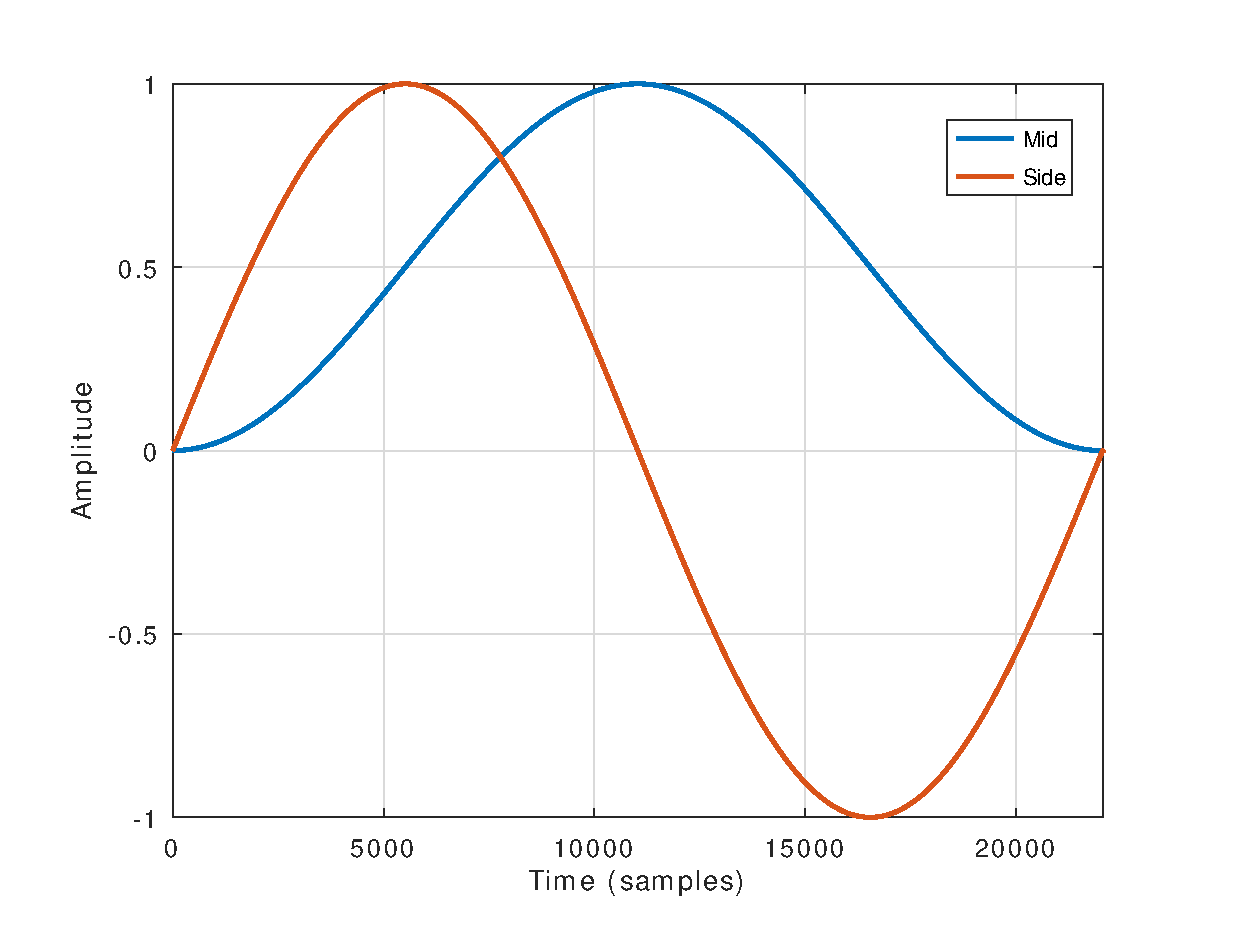
\includegraphics[width=1\columnwidth]{mspan}
% \caption{\textbf{Mid-Side Panner}. The plot shows the 360 degrees sweep from left -180 degrees to right 180 degrees. The Side (red) line shows the bipolarity of the signal related to the angular information. The Mid (blue) line has only positive energy in relation to angular information. The plot shows the evidence of the zero meaning at both edges of -180 and 180 degrees, where cardioid and figure-8 are hear-less.}
% \label{fig:mspan}
% \end{figure}
%
% \newpage
% %%%%%%%%%%%%%%%%%%%%%%%%%%%%%%%%%%%%%%%%%%%%%%%%%%%%%%%%%%%%%%%%%%%% SECTION SIX
% %%%%%%%%%%%%%%%%%%%%%%%%%%%%%%%%%%%%%%%%%%%%%%%%%%%%%%%%%%%%%%%%%%%%%%%%%%%%%%%%
% \section{Mid-Side Panner}
% \label{sec:mspanner}
%
% The following passages will lead step-by-step to the Mid-Side panner developing. First of all, it is necessary to understand the polar pattern significance of a signal. A single signal, in its amplitude variance around zero, could be derived by any kind of microphone without particular meaning. It could be electrically generated by a microphone or another synthetic source without specific relevance. The polar provenience, the shape of the signal phase, becomes relevant to the comparison between signals.
%
% From the Blumlein description of \emph{Mid-Side}, we have a \emph{Mid} frontal channel commonly described by a cardioid microphone. The first-order cardioid microphone could be described as a sum of non-directional pressure (\emph{ndp}) variations
%
% \begin{equation}
% ndp = 1(x)
% \label{eq:omni}
% \end{equation}
%
% and bidirectional pressure gradient variations.
%
% \begin{equation}
% bpg = x\cos\theta
% \label{eq:fig8}
% \end{equation}
%
% The first relevant difference between a non-directional polar pattern equation (\ref{eq:omni}) and directional one (\ref{eq:fig8}) is the presence of the angular coefficient. The \emph{theta} angle in the equation (\ref{eq:fig8}) describes the pointing direction of the bidirectional microphone expressed in radians. The $x$ is the pressure relative signal.
%
% The cardioid (\emph{cpg}) microphone we attempt to synthesize must point to the front-central position that is the zero radians reference.
%
% \begin{equation}
% cpg = 0.5(x) + 0.5(x\cos\theta)
% \label{eq:cardioid}
% \end{equation}
%
% Cardioid and other first-order most common patterns are produced with the following weight  between non-directional pressure and bidirectional pressure gradient:
%
% \begin{table}[h]
% \begin{center}
% \begin{tabular}{cc}
% Polar Pattern & Equation \\
% \hline
% Omnidirectional & $ 1(x) $ \\
% Subcardioid     & $ 0.75(x) + 0.25(x\cos\theta) $ \\
% Cardioid        & $ 0.5(x) + 0.5(x\cos\theta) $ \\
% Supercardioid   & $ 0.37(x) + 0.63(x\cos\theta) $ \\
% Hypercardioid   & $ 0.25(x) + 0.75(x\cos\theta) $ \\
% Bidirectional   & $ 1(x\cos\theta) $ \\
% \end{tabular}
% \end{center}
% \caption{\emph{non-directional pressure} coefficient and \emph{bidirectional pressure gradient} coefficient to first order polar patterns description. Where the $x$ is the input signal, the $\theta$ perspective angle of incidence}
% \label{tab:example}
% \end{table}
%
% So by the primitive first-order polar patterns, non-directional and bidirectional, we could derive, progressively, each shade of shape between them, angular pointing everywhere around 2$\pi$ radians.
%
% Finally, the Mid component of the Mid-Side panner could be expressed by the formula
%
% \begin{equation}
% m(x,p,\theta) = (p*x) + ((1-p)*(x\cos\theta)
% \label{eq:mid}
% \end{equation}
%
% Where $x$ is the input signal, the $p$ is the amplitude coefficient, $0.5$ for cardioid purpose, the $\theta$ is the angular impact direction expressed in radians.
%
% The Side component is the bipolar figure-8 straight formula pointing on left.
%
% \begin{equation}
% s(x,\theta) = x*(sin(\theta))
% \label{eq:mid}
% \end{equation}
%
% The Faust code for a Mid-Side panner is truly self-explained: the straight equations to describe both cardioid and figure-8 are the two components at the out of panning.
%
% %--------------------------------------------
% %----------------larghezza massima del codice
% \begin{lstlisting}
% mspan(x,p,rad) = m,s
% with{
%   m = (p*x)+((1-p)*(x*cos(rad)));
%   s = x*(sin(-rad));
% };
% \end{lstlisting}
%
%
% We must pass the panner through the sum-difference matrix to obtain what Blumlein describes as the difference of amplitude at loudspeakers signals from the differences of phases.
%
% %--------------------------------------------
% %----------------larghezza massima del codice
% \begin{lstlisting}
% mspan_lr(x,p,rad) = mspan(x,p,rad) : sdmx;
% \end{lstlisting}
%
% %\section{Floats and equations}
% %
% %\subsection{Equations}
% %Equations should be placed on separated lines and numbered. The number should be on the right side, in parentheses.
% %\begin{equation}
% %r=\sqrt[13]{3}
% %\label{eq:BP}
% %\end{equation}
% %Always refer to equations like this: ``Equation (\ref{eq:BP}) is of particular interest because...''
% %
% %\subsection{Figures, Tables and Captions}
% %\begin{table}[t]
% % \begin{center}
% % \begin{tabular}{|l|l|}
% %  \hline
% %  String value & Numeric value \\
% %  \hline
% %  Moin! SMC & 2020 \\
% %  \hline
% % \end{tabular}
% %\end{center}
% % \caption{Table captions should be placed below the table,  like this.}
% % \label{tab:example}
% %\end{table}
% %
% %All artwork must be centered, neat, clean and legible. Figures should be centered, neat, clean
% %and completely legible. All lines should be thick and dark enough for purposes of reproduction. Artwork should not be hand-drawn. The proceedings will be distributed in electronic form only, therefore color figures are allowed. However, you may want to check that your figures are understandable even if they are printed in black-and-white.
% %
% %
% %Numbers and captions of figures and tables always appear below the figure/table.
% %Leave 1 line space between the figure or table and the caption.
% %Figure and tables are numbered consecutively.
% %Captions should be Times 10pt. Place tables/figures in the text as close to the reference as possible,
% %and preferably at the top of the page.
% %
% %Always refer to tables and figures in the main text, for example: ``see Fig. \ref{fig:example} and \tabref{tab:example}''.
% %Figures and tables may extend across both columns to a maximum width of 17.2cm.
% %
% %Vectorial figures are preferred, e.g., eps. When using \texttt{Matlab}, export using either (encapsulated) Postscript or PDF format. In order to optimize readability, the font size of text within a figure should be no smaller than
% %that of footnotes (8~pt font-size). If you use bitmap figures, make sure that the resolution is high enough for print quality.
%
% \begin{figure}[h]
% \centering
% 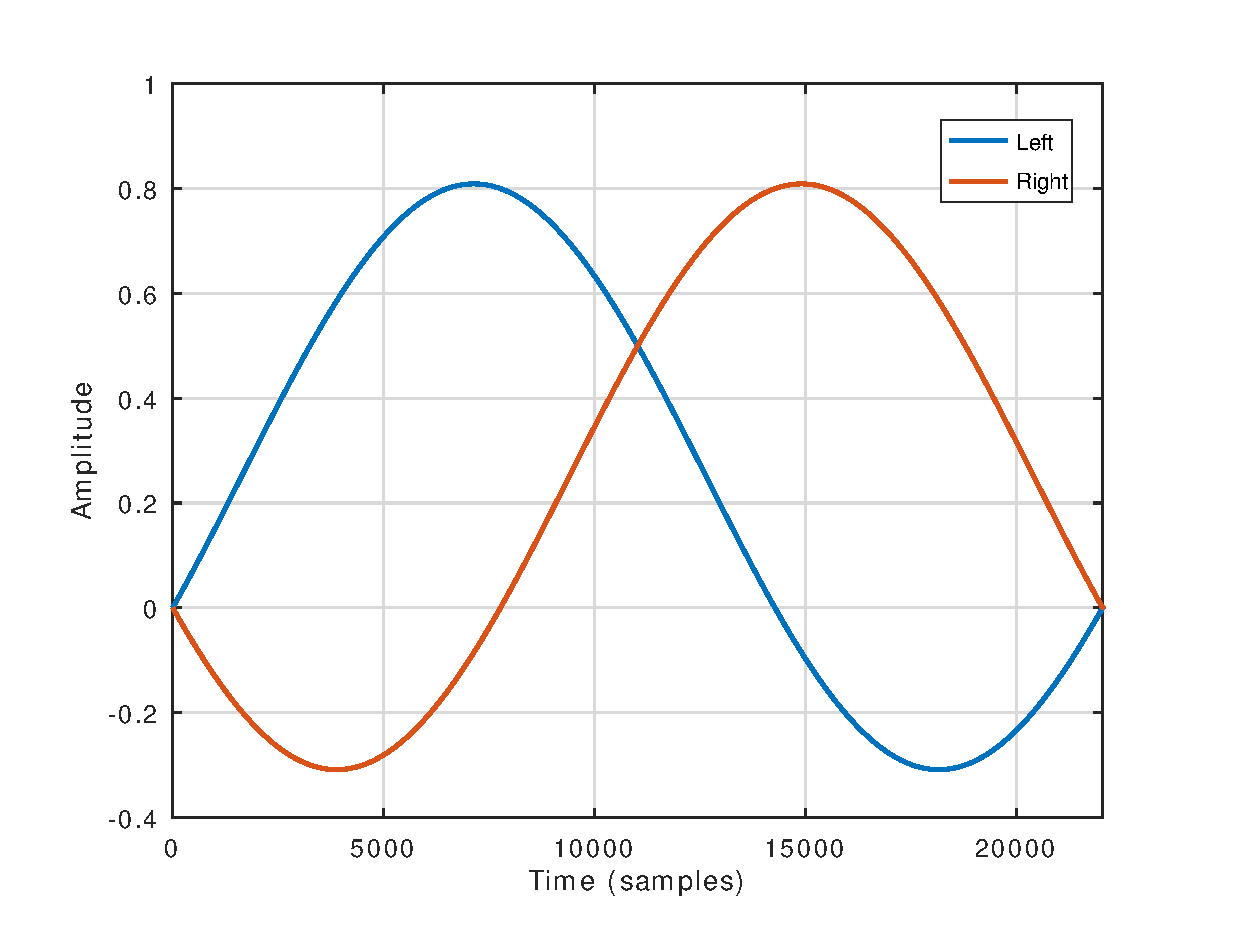
\includegraphics[width=1\columnwidth]{mspanlr}
% \caption{\textbf{Mid-Side Panner to Left-Right amplitude}. The plot shows the 360 degrees sweep from left -180 degrees to right 180 degrees. The top amplitude with a cardioid polar pattern for the Mid channel is around 0.8. The 1 amplitude factor is reached when the Mid channel has an omnidirectional polar pattern. The plot shows the negative amplitude at opposite angular provenience }
% \label{fig:mspanlr}
% \end{figure}
%
% % %\vfill\null
% % %
% % %\newpage
% % %%%%%%%%%%%%%%%%%%%%%%%%%%%%%%%%%%%%%%%%%%%%%%%%%%%%%%%%%%%%%%%%%% SECTION EIGHT
% % %%%%%%%%%%%%%%%%%%%%%%%%%%%%%%%%%%%%%%%%%%%%%%%%%%%%%%%%%%%%%%%%%%%%%%%%%%%%%%%%
% %
% % \section{MS-PAN Live usage}
% % \label{sec:mspanlive}
% %
% % The Mid-Side panner here proposed is not only a technical object, useful or not, comparable or not, related to other pan-kind. The Mid-Side panner here proposed is an object of thinking. We use the Mid-Side technique, to reflect stereophony itself; because we strongly think that some circumstances highlighted in previous sections need to be approached, others improved and many others killed.
% %
% % Thinking about panning must be strongly encouraged because it is a simple object too often used without questioning. People can think that the quadratic panner is better than the linear one that only by virtue its most recent introduction. But if we stop its “usage without questioning” and, as musicians, we take time to analyse the manual usage of one in place of the other we can feel a difference, practical before sonic.
% %
% % By knowing them we can analyse the mixer market and the role of panning in mass-culture music. Without an\-a\-lys\-ing these practical issues, it is not really understandable why the worst panning technique ever is the most hardware implemented.
% %
% % The code to build a quadratic amplitude panner is pretty trivial.
% % The most prolix \emph{Faust} code will do it in five lines. Deleting the $sqrt$ from the following formulas it becomes the simplest traditional linear amplitude panner.
% %
% % %--------------------------------------------
% % %----------------larghezza massima del codice
% % \begin{lstlisting}
% % lrpanq(x,p) = l,r
% % with{
% %   l = sqrt(1-p)*x;
% %   r = sqrt(p)*x;
% % };
% % \end{lstlisting}
% %
% % Where $p$ is the angular coefficient expressed by the potentiometer, in a range between $0$ the Left position, $0.5$ the Center position and $1$ the Right position.
% %
% % Smiling, it could be done by one line:
% %
% % %--------------------------------------------
% % %----------------larghezza massima del codice
% % \begin{lstlisting}
% % lrpanq(p) = _ <: sqrt(1-p)*_, sqrt(p)*_;
% % \end{lstlisting}
% %
% % \begin{figure}[t]
% % \centering
% % 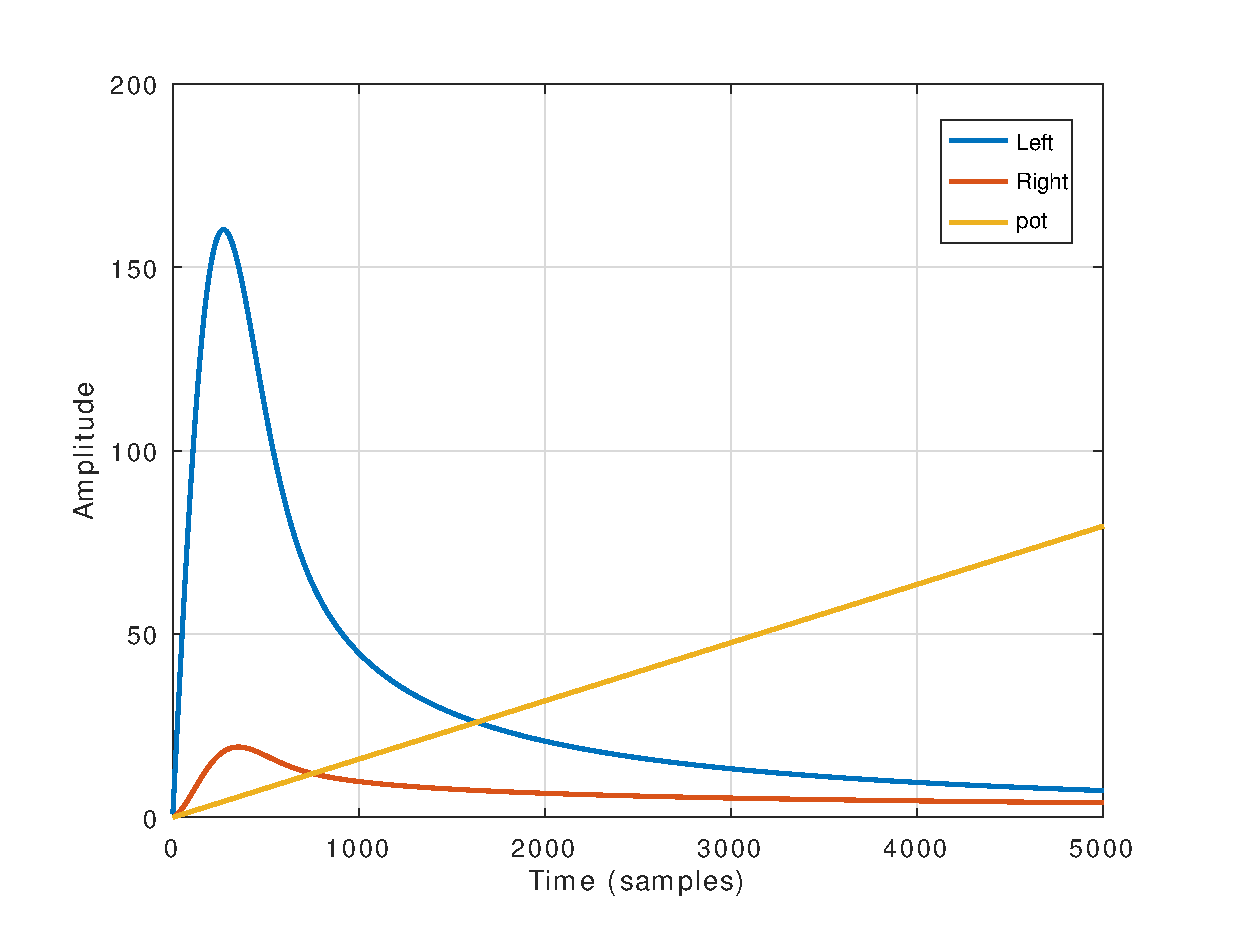
\includegraphics[width=1\columnwidth]{lrpanfb_init}
% % \caption{\textbf{Left-Right quadratic amplitude panner feedback response}. The plot shows panner response at one cycle of sweep from left to right. The plot shows as amplitude moves fast over 150 times the initial value on the “in-feedback” channel and over 20 times on the “opposite” channel.}
% % \label{fig:lrpanfb1}
% % \end{figure}
% %
% % \begin{figure}[t]
% % \centering
% % 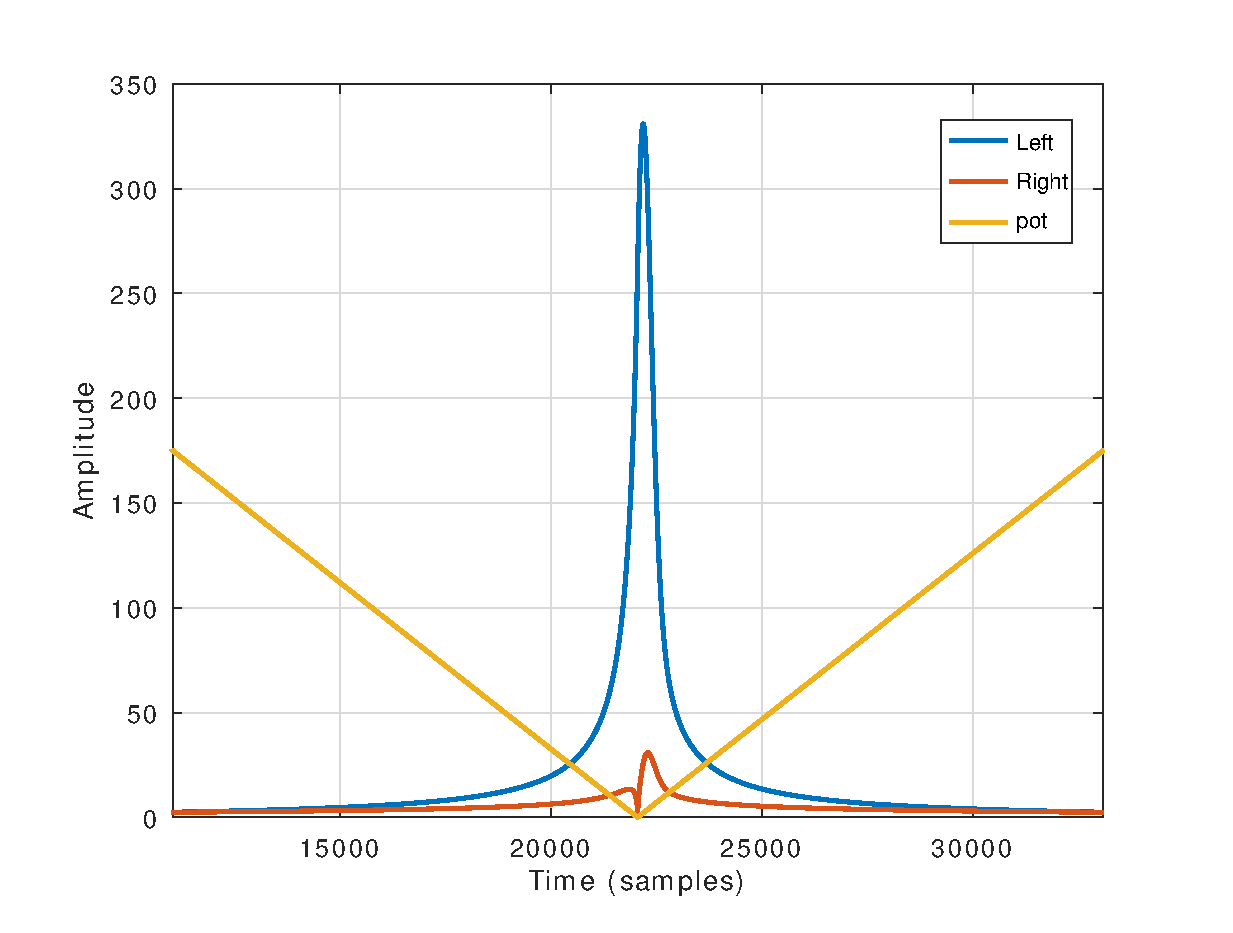
\includegraphics[width=1\columnwidth]{lrpanfbpot2}
% % \caption{\textbf{Left-Right quadratic amplitude panner feedback response}. The plot shows the moment in which the cycle of sweep pass from right through left and again reversing to right. It shows as amplitude moves fast over 300 times the initial value on the “in-feedback” channel and over 30 times on the “opposite” channel.}
% % \label{fig:lrpanfb2}
% % \end{figure}
% %
% % We have explained the path to Mid-Side panning, starting from the roots. Now it is the moment to understand what are the possible usages and what are the peculiarities of a Mid-Side panner instead of the \emph{traditional} amplitude panners.
% %
% % The \emph{matrixed} signal has its complexity as a disadvantage. Stop. In fact it requires knowledge and fantasy to understand a signal as the significance of matrix combination and it also requires a bit of tricky work more than a straight-signal.
% %
% % As musicians, even when plots and formulas appear pretty clear, in the end, at the moment of judgment, are the ears and the musical usability to determine the best, personal, choice.
% %
% % The fascinating realm of \emph{matrixed} signals forces a little to work by thought. So, for us, for example, the phase modulation strength of the Mid-Side panner had suggested, even before a practical test, better stability on live usages. Why? It is pretty simple to demonstrate.
% %
% % A microphone is routed into a channel, with a mid-lateral pointed panner, suppose 23 degrees to left and fed to the loudspeakers. With the quadratic panner, both left and right channels have different amplitude values with the same phase values. The feedback of the loudspeakers' signals inside the microphone comes from in-phase different energies sources. Searching the feedback with fingers on the gain will produce signals that will increase at least quadratically [fig. \ref{fig:lrpanfb1}, \ref{fig:lrpanfb2}].
% %
% % \begin{figure}[h]
% % \centering
% % 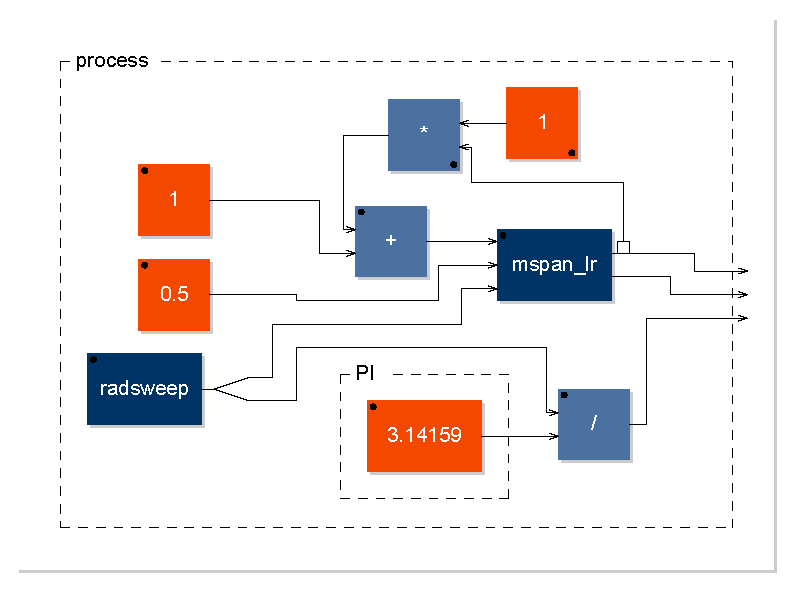
\includegraphics[width=1\columnwidth]{mspanlrfb_diagram}
% % \caption{\textbf{Block diagram of the infinite feedback}.}
% % \label{fig:mspan}
% % \end{figure}
% %
% % On the other hand, in the same feedback situation, with the same angular panning provenience applied to the microphone signal, the Mid-Side panning will produce different phase and different energy for both loudspeakers. The differences, in air, will produce a more resistive feedback pattern. In other words, the Mid-Side panner act "naturally" as anti-\emph{Larsen}.
% %
% % %\vfill\null
% % %\newpage
% %
% % %%%%%%%%%%%%%%%%%%%%%%%%%%%%%%%%%%%%%%%%%%%%%%%%%%%%%%%%%%%%%%%%%% SECTION SEVEN
% % %%%%%%%%%%%%%%%%%%%%%%%%%%%%%%%%%%%%%%%%%%%%%%%%%%%%%%%%%%%%%%%%%%%%%%%%%%%%%%%%
% % \section{CONCLUSIONS}
% % \label{sec:conc}
% %
% % \begin{figure}[t]
% % \centering
% % 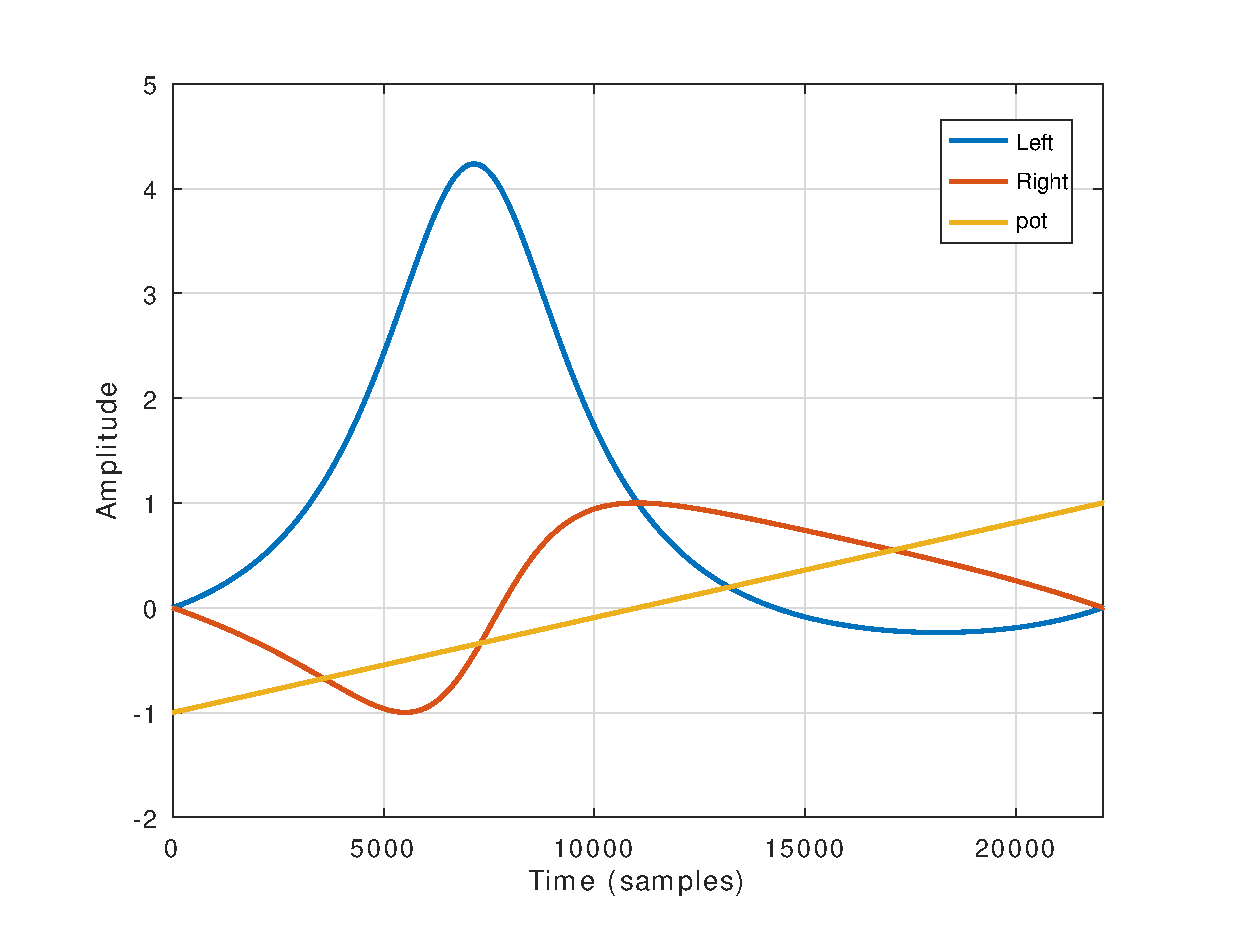
\includegraphics[width=1\columnwidth]{mspanlrfbpot}
% % \caption{\textbf{Mid-Side to Left-Right panner}. The plot describes the feedback response with a pan movement through the entire panorama, from -180 to 180 degrees (yellow line, normalized to -1 and 1). The energy multiplies up to four times for the left channel in infinite feedback (blue line). The top of feedback increasing is at 45 degrees position in direction of the channel in feedback.}
% % \label{fig:mspanlrfb}
% % \end{figure}
% %
% % This is the second article \emph{SEAM} produces to spread the music sustainability concept \cite{bevi05} from live electronics music to the broader electroacoustic music composition and interpretation. The original issues about music score documentation in electronic music are the fundamental core of the concept. Nevertheless, the focus of this research, and the approach, point to a compositional and practical situation that afflicts not only the documentation of a score but the musical thinking and practice at all.
% %
% % The research defines a critical educational situation, the first one analysed pretend to overcome literature with a new fancy way of teaching, writing books, in our opinion ludic, to educate like playing. There are a lot of textbooks, didactically introduced at each level of electronic music school, with the “doing, does not matter why" approach. You can pretty simply recognize them, they offer electronic music teaching as a collection of recipes, articulated like a foreign language book. Some authors praise themselves for the didactic unit-based structure of their books, inspired by foreign language learning texts. Is that music? Is music a foreign language? From these gruesome attitudes, the \emph{SEAM PROJECT} wants to take long-distance. What distance? Distance in thinking music and thinking about music, because sustainability is only superficially a technical issue. The documentation is a quality parameter of sustainability but it is the musical practicing and interpreting that will build musical thinking during the years.
% %
% % The first concept to be clarified in the conclusions is that sustainability must aim at maintaining a musical idea, the peculiarities of a concept is necessary like the peculiarities of the piece of art. We point at sustaining the speculation that music produces, through the sustaining of listening, that we have defined as the \emph{sustainability of the process}.
% %
% % %The paper also has a journey profile, conceived around the idea of speaking diagonally to different levels of electroacoustic learning.  The repertoire, the literature, needs people sharing their knowledge, to refine common conscience. A community can operate as a Research Group, with a “common appreciation of interdisciplinary problems” \cite{ml91}, to bring a time-frozen composition back to a warm and discussed work, out of a solipsistic production-in-a-box typical of the personal computing era, to focus on musical matters carved out on the personal knowledge, outside the personal point of view.
% %
% % It is necessary to focus on the main difference between technical sustainability and musical sustainability. Technical sustainability concerns the work, it is linked to the technical world that the work defines. It is its carbon dating, the reproducible ecosystem, maybe, but it is not the work itself. Musical sustainability is a matter of thoughts, that makes use of those tools to go out towards the perceptible. Supporting the thoughts is supporting music, perception, and listening.
% %
% % \begin{quote}
% % La musica non è solo composizione. Non è artigianato, non è un mestiere. La musica è pensiero \cite{nono85}\footnote{Music is not only about composing. It’s not handcraft, neither only a craft. Music is thought.}.
% % \end{quote}
